\chapter{糖类}\label{ch:b1:carbohydrates}

马铃薯与一张纸，都由同一种分子——葡萄糖——
串联成链。一种是食物，另一种不是，原因在于
两者的链由两种不同的键连接：\omterm{def:b1:carbohydrates:polysaccharide}{淀粉}中的 $\alpha$ 键
使链卷曲成螺旋，我们的酶能将其打开；\omterm{def:b1:carbohydrates:polysaccharide}{纤维素}中的 $\beta$ 键
使链伸展成带状，这些带状结构堆叠成纤维，没有哺乳动物能够消化。
肝脏以\omterm{def:b1:carbohydrates:polysaccharide}{糖原}的形式储存一百克葡萄糖，树木
依靠\omterm{def:b1:carbohydrates:polysaccharide}{纤维素}支撑自身，甲虫披着\omterm{def:b1:carbohydrates:polysaccharide}{几丁质}外壳，而每个
\omterm{def:b1:cell-unit-of-life:cell}{细胞}都在表面展示\omterm{def:b1:carbohydrates:monosaccharide}{糖类}作为其身份标识。本章介绍\omterm{def:b1:carbohydrates:monosaccharide}{单糖}、
连接\omterm{def:b1:carbohydrates:monosaccharide}{单糖}的\omterm{def:b1:carbohydrates:glycosidic}{糖苷键}、
由它们构成的\omterm{def:b1:carbohydrates:polysaccharide}{多糖}，
以及\omterm{def:b1:cell-unit-of-life:cell}{细胞}表面和植物\omterm{def:b1:eukaryotic-cell:plantcell}{细胞壁}上带糖修饰的分子。

\section{单糖}

\begin{definition}[单糖]\label{def:b1:carbohydrates:monosaccharide}
\emph{糖类}\index{糖类}是组成为
$(\mathrm{CH_2O})_n$ 的分子及其衍生物。
\emph{单糖}\index{单糖}（简单糖）是一条碳链，
长三至七个碳原子，其中一个碳带羰基，其余碳带羟基：
羰基位于链端时为\emph{醛糖}\index{醛糖}，
即醛，例如葡萄糖、半乳糖、核糖；羰基位于链内
时为\emph{酮糖}\index{酮糖}，即酮，例如果糖。
按碳原子数分类：丙糖（$n = 3$，甘油醛）、戊糖（$n = 5$，
核糖、脱氧核糖），己糖（$n = 6$，葡萄糖、果糖、半乳糖）。
每个连有四个不同基团的碳都是\emph{手性}中心，
因此每个分子式代表若干种\emph{立体异构体}：葡萄糖有四个手性碳，
共十六种异构体，\omterm{def:b1:organism-environment:organism}{生物体}只利用其中一种，
即 D-葡萄糖。\emph{差向异构体}仅在一个碳原子上不同（葡萄糖与
半乳糖在 C4 处不同）。
\end{definition}

\begin{proposition}[环式结构与异头物]\label{prop:b1:carbohydrates:rings}
\index{异头物}\index{哈沃斯投影式}
在水中，戊糖或己糖几乎全部以环状存在：羰基
碳与同一分子中的羟基（葡萄糖中为 C5 上的羟基）反应，
闭合成六元\emph{吡喃糖}环或五元
\emph{呋喃糖}环（果糖、核糖）。羰基碳成为
新的手性中心，即\emph{异头碳}，其羟基可位于
环平面下方（$\alpha$ 异头物）或上方（$\beta$ 异头物）
哈沃斯投影图中；两种形式经开链结构
在数分钟内相互转化。溶液中，葡萄糖为\qty{36}{\%}的 $\alpha$ 型、\qty{64}{\%}
$\beta$ 型，开链结构不足\qty{0.1}{\%}。游离的异头碳
是使糖具有\emph{还原性}的原因：它能开环，
并还原铜试剂或银试剂。
\end{proposition}

\begin{omfigure}
\begin{tikzpicture}[font=\footnotesize, line cap=round, line join=round]
  \newcommand{\haworth}[2]{%
    % ring: C5 top-left, O top-right, C1 right, C2 bottom-right, C3 bottom-left, C4 left (scaled 1.4)
    \draw[thick] (0.84,1.54) -- (2.52,1.54) -- (3.64,0.42) -- (2.52,-0.7) -- (0.84,-0.7) -- (-0.28,0.42) -- cycle;
    \draw[line width=3.5pt] (0.84,-0.7) -- (2.52,-0.7);
    \draw[line width=2.5pt] (2.52,-0.7) -- (3.64,0.42);
    \draw[line width=2.5pt] (0.84,-0.7) -- (-0.28,0.42);
    \node[fill=white, inner sep=1pt] at (2.52,1.54) {O};
    \node[font=\scriptsize] at (3.25,0.42) {1};
    \node[font=\scriptsize] at (2.45,-0.35) {2};
    \node[font=\scriptsize] at (0.9,-0.35) {3};
    \node[font=\scriptsize] at (0.1,0.42) {4};
    \node[font=\scriptsize] at (0.95,1.2) {5};
    % C5: CH2OH up
    \draw (0.84,1.54) -- (0.84,2.2) node[above] {$\mathrm{CH_2OH}$};
    % C4: OH down, H up
    \draw (-0.28,0.42) -- (-0.28,1.05) node[above] {H};
    \draw (-0.28,0.42) -- (-0.28,-0.2) node[below] {OH};
    % C3: OH up
    \draw (0.84,-0.7) -- (0.84,-0.05) node[above, xshift=-3pt] {OH};
    \draw (0.84,-0.7) -- (0.84,-1.3) node[below] {H};
    % C2: OH down
    \draw (2.52,-0.7) -- (2.52,-1.3) node[below] {OH};
    \draw (2.52,-0.7) -- (2.52,-0.05) node[above, xshift=3pt] {H};
    % C1: anomeric
    \draw (3.64,0.42) -- (3.64,1.05) node[above] {#1};
    \draw (3.64,0.42) -- (3.64,-0.2) node[below] {#2};
  }
  \begin{scope}
    \haworth{H}{OH}
    \node[anchor=north, align=center] at (1.7,-1.9) {$\alpha$-D-葡萄糖 \\ 异头羟基（1号碳）在环下方};
  \end{scope}
  \begin{scope}[xshift=8.4cm]
    \haworth{OH}{H}
    \node[anchor=north, align=center] at (1.7,-1.9) {$\beta$-D-葡萄糖 \\ 异头羟基（1号碳）在环上方};
  \end{scope}
  \draw[<->, thick, gray] (4.9,0.42) -- (7.4,0.42) node[midway, above, align=center] {开链 \\ （醛式）};
\end{tikzpicture}

{\small D-葡萄糖两种异头物的哈沃斯投影：环以侧视方式呈现，
较粗的一边朝向读者，异头碳（1号碳）上的羟基
位于平面下方（$\alpha$）或上方（$\beta$）。二者
经开链醛式结构相互转化。}
\end{omfigure}

\begin{method}[读懂哈沃斯投影]\label{met:b1:carbohydrates:haworth}
\begin{enumerate}
  \item 找到环中的氧原子；异头碳（\omterm{def:b1:carbohydrates:monosaccharide}{醛糖}中为 C1，
        \omterm{def:b1:carbohydrates:monosaccharide}{酮糖}中为 C2）是其右侧的环碳，同时带有
        一个羟基和环中的氧原子。
  \item 环外带有 $\mathrm{CH_2OH}$ 基团的碳
        （葡萄糖中为 C5）位于环中氧原子的左侧；其
        $\mathrm{CH_2OH}$ 在 D 型糖中朝上。
  \item 异头羟基朝下为 $\alpha$；朝上（与
        $\mathrm{CH_2OH}$ 同侧）为 $\beta$。
  \item 将其余羟基与葡萄糖的对应羟基比较（分别为下、上、
        下，对应 C2、C3、C4）：仅一处不同即可判定为差向异构体
        （半乳糖：C4 朝上）。
\end{enumerate}
\end{method}

\begin{example}[不是 $(\mathrm{CH_2O})_n$ 的糖]\label{ex:b1:carbohydrates:derivatives}
脱氧核糖的 C2 上缺少羟基（见\cref{ch:b1:nucleic-acids}）；
葡糖胺和 N-乙酰葡糖胺以氨基代替 C2 上的
羟基（见于\omterm{def:b1:carbohydrates:polysaccharide}{几丁质}、\omterm{def:b1:carbohydrates:polysaccharide}{肽聚糖}）；葡糖醛酸在 C6 上带有羧基
（见于基质\omterm{def:b1:carbohydrates:polysaccharide}{多糖}）；糖磷酸（6-磷酸葡萄糖、
5-磷酸核糖）是糖进入代谢的形式；
糖醇（甘油、山梨醇）不含羰基。其核心相同：
一条带有多个羟基的小型碳链，亲水。
\end{example}

\section{糖苷键}

\begin{definition}[糖苷键，二糖]\label{def:b1:carbohydrates:glycosidic}
\emph{糖苷键}\index{糖苷键}将一个糖的异头
羟基与另一糖（或醇、胺、碱基）的羟基相连，
通过\omterm{prop:b1:water-small-molecules:families}{缩合}，使异头碳固定为
$\alpha$ 或 $\beta$ 构型；其命名由构型及所连碳决定：
$\alpha(1{\to}4)$、$\beta(1{\to}4)$、
$\alpha(1{\to}6)$。两个糖以此方式相连，
形成\emph{二糖}\index{二糖}：\emph{麦芽糖}
（葡萄糖 $\alpha(1{\to}4)$ 葡萄糖，由\omterm{def:b1:carbohydrates:polysaccharide}{淀粉}消化产生），
\emph{乳糖}（半乳糖 $\beta(1{\to}4)$ 葡萄糖，即乳汁中的糖），
\emph{蔗糖}（葡萄糖 $\alpha(1{\to}2)\beta$ 果糖，即
植物汁液和厨房中的糖）。蔗糖中两个异头碳均
参与成键，它为非还原糖、不开环，这正是植物
运输它的原因（见\cref{ch:b1:plant-transport}）。
\end{definition}

\begin{method}[检验还原糖]\label{met:b1:carbohydrates:reducing}
\begin{enumerate}
  \item 用碱性铜(II)试剂加热溶液
        （本尼迪特试剂或费林试剂）。
  \item 游离的异头碳开环生成醛，将蓝色的
        $\mathrm{Cu^{2+}}$ 还原为砖红色的 $\mathrm{Cu_2O}$ 沉淀；
        颜色深浅与糖的量成正比。
  \item 葡萄糖、果糖、麦芽糖、乳糖：阳性。蔗糖：阴性
——除非先经酸或转化酶水解，
        之后其葡萄糖和果糖即发生反应。
  \item \omterm{def:b1:carbohydrates:polysaccharide}{淀粉}不发生反应（其还原端在数千
        个残基中仅有一个）；可用碘检测，碘进入
        直链\omterm{def:b1:carbohydrates:polysaccharide}{淀粉}的螺旋，呈蓝黑色。
\end{enumerate}
\end{method}

\section{多糖}

\begin{definition}[多糖]\label{def:b1:carbohydrates:polysaccharide}
\emph{多糖}\index{多糖}是由数百至
数万个\omterm{def:b1:carbohydrates:monosaccharide}{单糖}通过\omterm{def:b1:carbohydrates:glycosidic}{糖苷键}连接而成的链，可为线性
或分支的。贮藏多糖：植物中的\emph{淀粉}\index{淀粉}
——\emph{直链淀粉}，无分支的 $\alpha(1{\to}4)$ 葡萄糖，
占 \qty{20}{\%}；\emph{支链淀粉}，为 $\alpha(1{\to}4)$ 连接，每
隔 \qtyrange{24}{30}{} 个残基有一个 $\alpha(1{\to}6)$ 分支，
占 \qty{80}{\%}，成颗粒储存；\emph{糖原}\index{糖原}见于
动物和真菌中，结构与支链淀粉相似，但每隔
\qtyrange{8}{12}{} 个残基即有分支，颗粒存在于肝脏和
肌肉的\omterm{def:b1:eukaryotic-cell:organelle}{细胞溶胶}中。结构性多糖：\emph{纤维素}\index{纤维素}，
无分支的 $\beta(1{\to}4)$ 葡萄糖链，含 \qtyrange{2000}{15000}{} 个残基，
存在于植物\omterm{def:b1:eukaryotic-cell:plantcell}{细胞壁}中；\emph{几丁质}\index{几丁质}，$\beta(1{\to}4)$
N-乙酰葡糖胺，存在于真菌\omterm{def:b1:eukaryotic-cell:plantcell}{细胞壁}和节肢动物的
\omterm{def:b1:flowering-plant-organization:tissues}{角质层}中；\emph{肽聚糖}\index{肽聚糖}，由
N-乙酰葡糖胺与 N-乙酰胞壁酸交替排列，并由短
肽交联，构成细菌\omterm{def:b1:eukaryotic-cell:plantcell}{细胞壁}的单分子网状结构。
\end{definition}

\begin{proposition}[糖苷键决定形状，形状决定功能]\label{prop:b1:carbohydrates:alphabeta}
在 $\alpha(1{\to}4)$ 链中，每个葡萄糖的朝向
均与前一个相同，链卷曲成每圈六个残基的螺旋，
开放、含水的螺圈，酶易于进入：这是一种
\emph{贮藏}的形式。在 $\beta(1{\to}4)$ 链中，每个葡萄糖
相对于其相邻残基翻转 $180^\circ$，链呈笔直的
平带状；带状链并排排列，通过\omterm{def:b1:water-small-molecules:water}{氢键}形成
由三十至一百条链组成的\emph{微纤丝}，结晶状、
不溶于水，单位质量的抗张强度与钢相当：这是
\emph{纤维}的形式。水解 $\alpha$ 键的酶（\omterm{def:b1:carbohydrates:polysaccharide}{淀粉}酶）
不能作用于 $\beta$ 键；\emph{\omterm{def:b1:carbohydrates:polysaccharide}{纤维素}酶}存在于细菌、真菌
及少数动物中，以草为食的哺乳动物则借助
共生菌实现消化（见\cref{ch:b1:digestion-absorption}）。
\end{proposition}

\begin{omfigure}
\begin{tikzpicture}[font=\footnotesize, line cap=round]
  % alpha helix: a coil drawn as a sequence of hexagons along a helix path
  \begin{scope}
    \draw[very thick, omProp, domain=0:1080, samples=240, smooth, variable=\t] plot ({1.0*cos(\t)}, {0.4*sin(\t)+0.0028*\t});
    \foreach \t in {0,60,...,1080} { \fill[omProp!70!black] ({1.0*cos(\t)}, {0.4*sin(\t)+0.0028*\t}) circle (0.09); }
    \draw[dashed, gray] (0,-0.6) -- (0,3.6);
    \node[anchor=north, align=center] at (0,-0.7) {$\alpha(1{\to}4)$：直链淀粉、糖原 \\ 每个残基朝向相同 \\ $\to$ 螺旋，每圈六个残基 \\ 开放、含水、易于消化};
  \end{scope}
  % beta ribbons: straight chains of alternating flipped hexagons, stacked
  \begin{scope}[xshift=6.0cm]
    \foreach \y in {0,0.9,1.8} {
      \draw[very thick, omDef] (0,\y) -- (5.0,\y);
      \foreach \i in {0,...,9} {
        \pgfmathsetmacro{\s}{ifthenelse(mod(\i,2)==0,1,-1)}
        \fill[omDef!70!black] (0.25+0.5*\i,\y) circle (0.08);
        \draw[omDef!70!black] (0.25+0.5*\i,\y) -- (0.25+0.5*\i,\y+0.22*\s);
      }
    }
    \foreach \x in {0.75,1.75,2.75,3.75,4.75} { \draw[dashed, gray] (\x,0.22) -- (\x,0.68) (\x,1.12) -- (\x,1.58); }
    \node[anchor=north, align=center] at (2.5,-0.7) {$\beta(1{\to}4)$：纤维素、几丁质 \\ 每个残基翻转 $180^\circ$\\ $\to$ 笔直的带状；带状链 \\ 通过氢键形成微纤丝};
  \end{scope}
\end{tikzpicture}

{\small 同一种葡萄糖，两种键，两类材料。左：
$\alpha(1{\to}4)$ 链卷曲成螺旋。右：$\beta(1{\to}4)$
链为平带状，相邻残基交替朝上、朝下；
相邻带状链通过（虚线所示的）\omterm{def:b1:water-small-molecules:water}{氢键}形成结晶状纤维。}
\end{omfigure}

\begin{omfigure}
\begin{minipage}[b]{0.44\linewidth}\centering
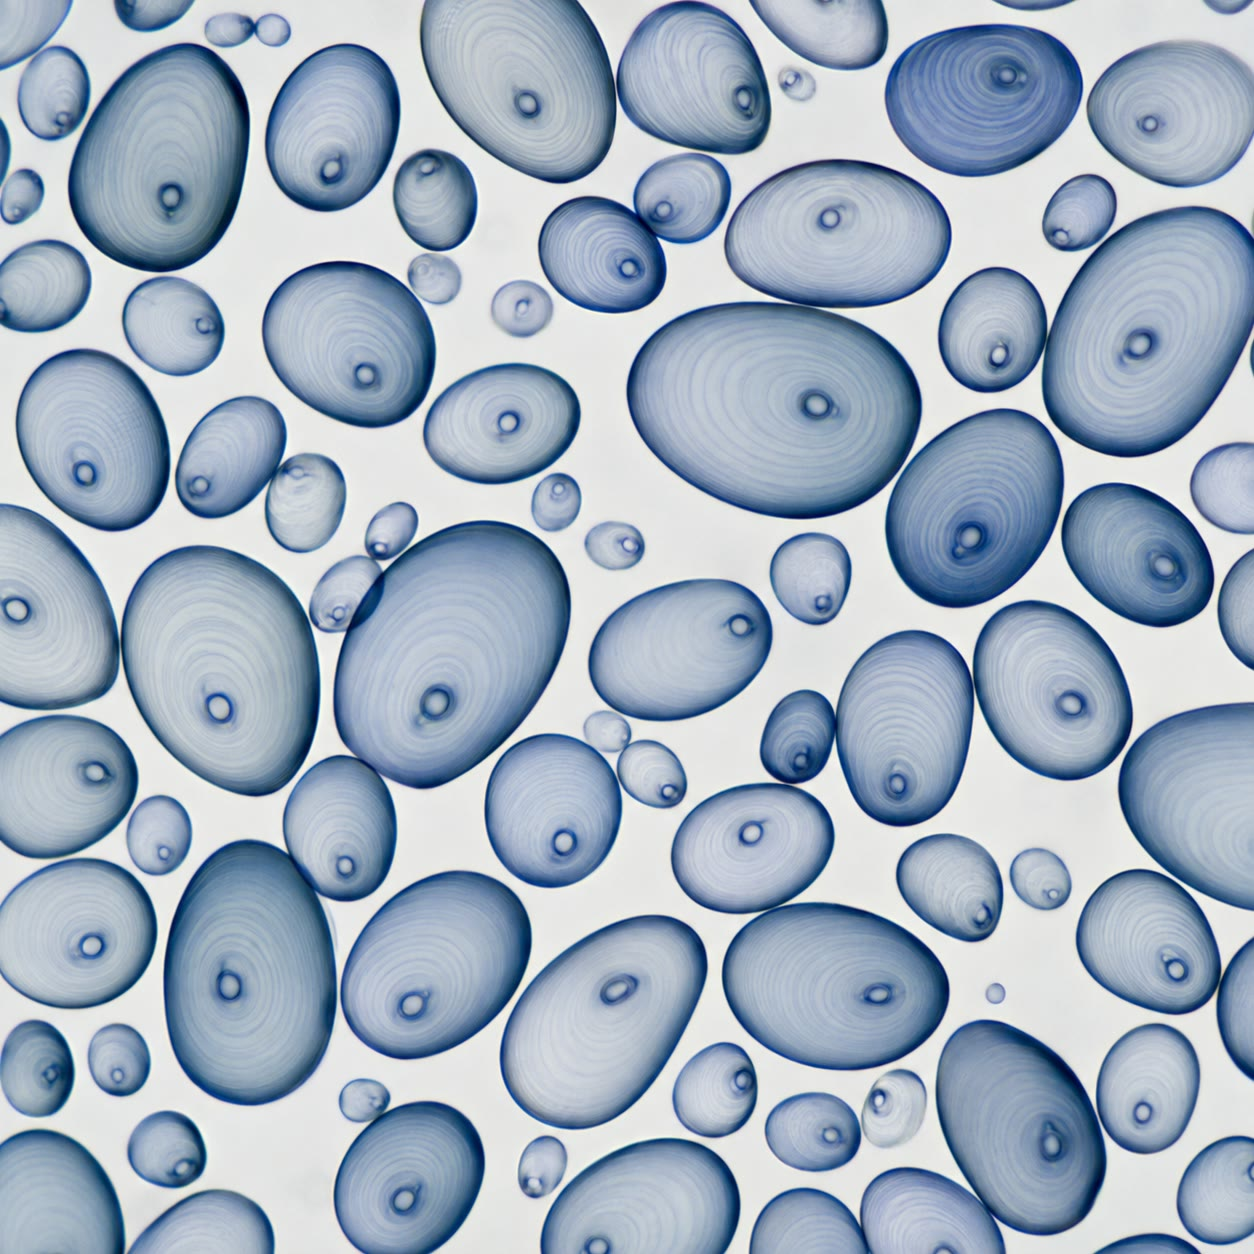
\includegraphics[width=0.96\linewidth]{images/book3/ai/b3-10-starch-grains.jpg}
\end{minipage}\hfill
\begin{minipage}[b]{0.52\linewidth}\centering
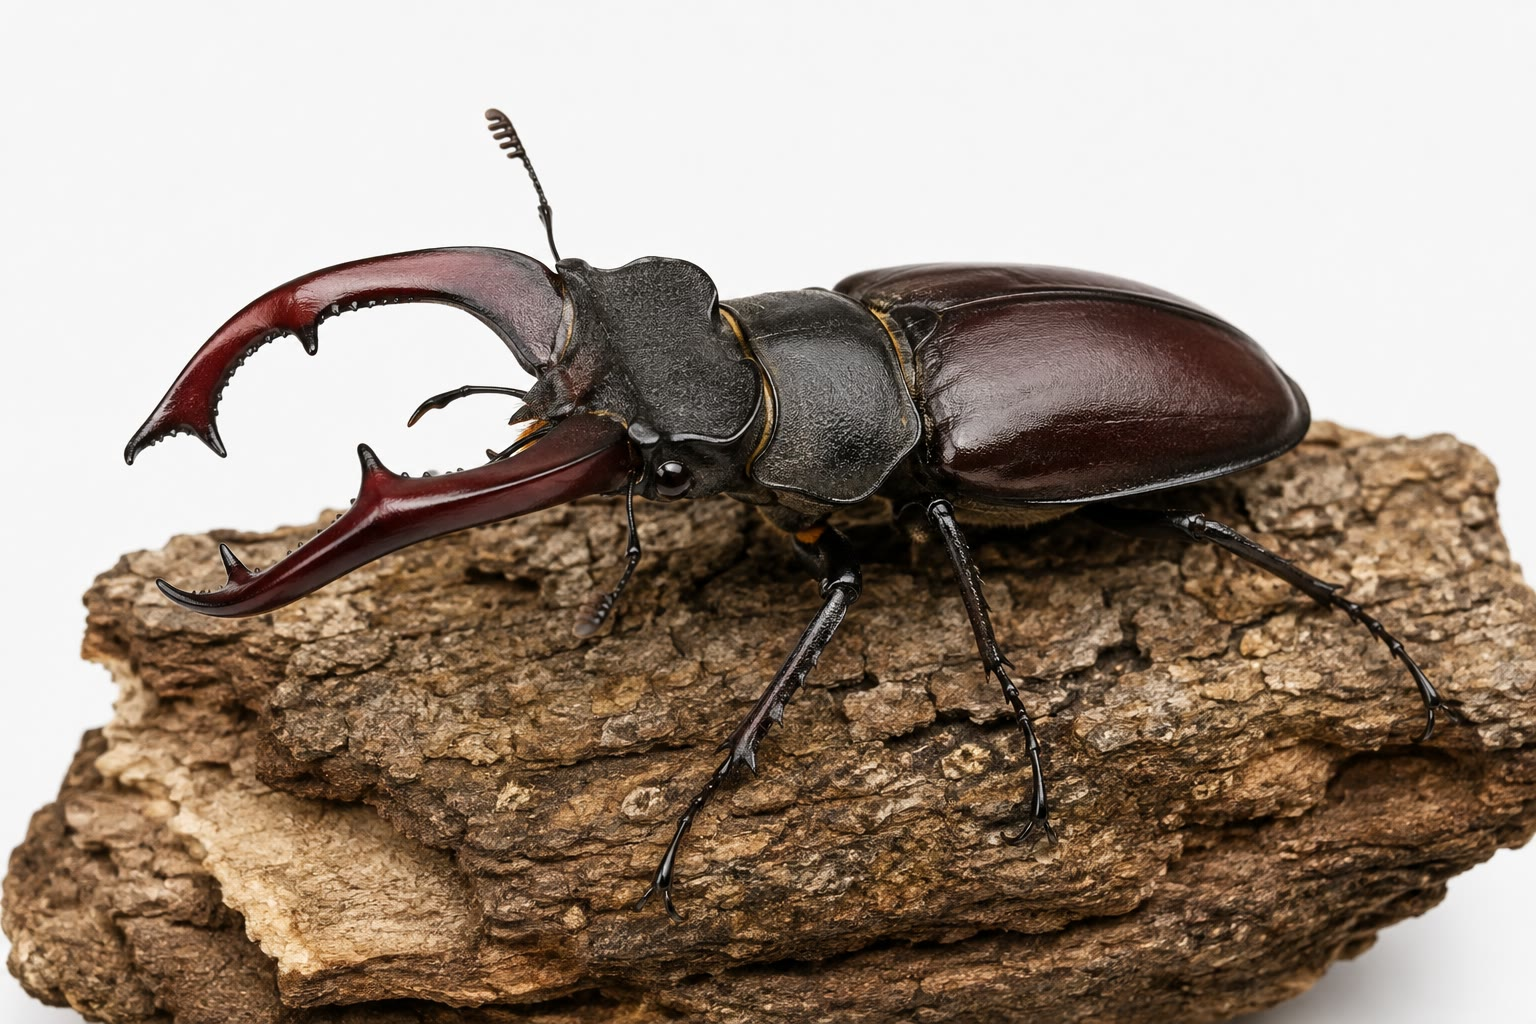
\includegraphics[width=0.96\linewidth]{images/book3/ai/b3-10-beetle-cuticle.jpg}
\end{minipage}

{\small 左：显微镜下的马铃薯\omterm{def:b1:carbohydrates:polysaccharide}{淀粉}粒，经碘染色；
同心环是逐日沉积的支链\omterm{def:b1:carbohydrates:polysaccharide}{淀粉}层。
右：锹甲的\omterm{def:b1:flowering-plant-organization:tissues}{角质层}——在蛋白质基质中的\omterm{def:b1:carbohydrates:polysaccharide}{几丁质}纤维，
坚硬而色深：与\omterm{def:b1:carbohydrates:polysaccharide}{纤维素}一样的 $\beta(1{\to}4)$ 设计，
只是糖的种类不同。}
\end{omfigure}

\begin{example}[糖原为何带分支]\label{ex:b1:carbohydrates:branching}
\omterm{def:b1:carbohydrates:polysaccharide}{糖原}从其非还原端降解，每次释放一个葡萄糖，
由\omterm{def:b1:carbohydrates:polysaccharide}{糖原}磷酸化酶催化。一条不分支、含 \num{50000} 个葡萄糖的链
只有一个这样的末端，每次酶周转只释放一个葡萄糖；
同样大小、每十二个残基分支一次的\omterm{def:b1:carbohydrates:polysaccharide}{糖原}颗粒，
约有 \num{2000} 个末端，可一次释放两千个。分支
还使颗粒保持紧凑并可溶。肝脏中的一百克
\omterm{def:b1:carbohydrates:polysaccharide}{糖原}可以每小时十克的速度动用；同样的葡萄糖
若以一条长链储存，则需数年才能解开。
\end{example}

\begin{example}[为何不直接储存葡萄糖]\label{ex:b1:carbohydrates:osmotic}
将一百克葡萄糖（\qty{0.55}{mol}）溶解于肝\omterm{def:b1:cell-unit-of-life:cell}{细胞}中的
\qty{1}{L} 水里，会使\omterm{def:b1:eukaryotic-cell:organelle}{细胞溶胶}的渗透浓度增加 \qty{0.55}{osmol/L}，
而其原有浓度为 \qty{0.3}{osmol/L}：\omterm{def:b1:cell-unit-of-life:cell}{细胞}将膨胀至原体积的三倍，
并破裂。若以\omterm{def:b1:carbohydrates:polysaccharide}{糖原}形式储存同样的葡萄糖，则为
$\num{7e18}$ 个粒子，浓度为 \qty{1e-5}{mol/L}，渗透上不可见。
聚合物是把大量分子储存为一个整体的方式。
\end{example}

\section{糖缀合物与植物细胞壁}

\begin{definition}[糖蛋白、蛋白聚糖、糖脂]\label{def:b1:carbohydrates:glycoconjugate}
糖以\omterm{def:b1:water-small-molecules:bonds}{共价键}与蛋白质和脂质相连，
形成\emph{糖缀合物}\index{糖缀合物}。\emph{糖蛋白}\index{糖蛋白}在其部分
天冬酰胺、丝氨酸或苏氨酸残基上
带有短的分支链（约十二个糖），
这些链在\omterm{def:b1:eukaryotic-cell:endomembrane}{内质网}和\omterm{def:b1:eukaryotic-cell:endomembrane}{高尔基体}中加上（见\cref{ch:b1:eukaryotic-cell}）：
几乎所有分泌蛋白和\omterm{def:b1:membranes-transport:membrane}{膜蛋白}都是糖蛋白。
\emph{蛋白聚糖}\index{蛋白聚糖}是以蛋白质为核心的分子，
其上带有长的不分支链，
链由重复的酸性\omterm{def:b1:carbohydrates:glycosidic}{二糖}单位组成，即\emph{糖胺聚糖}\index{糖胺聚糖}
（透明质酸、硫酸软骨素、肝素），它们结合大量的水，
使软骨、玻璃体和\omterm{def:b1:body-plans-tissues:connective}{细胞外基质}具有恢复力。
\emph{糖脂}\index{糖脂}位于\omterm{def:b1:membranes-transport:membrane}{质膜}外小叶的脂质尾部，带有糖。
糖脂与糖蛋白上的糖一起
构成\emph{糖萼}\index{糖萼}，即\omterm{def:b1:cell-unit-of-life:cell}{细胞}借以被\omterm{prop:b1:water-small-molecules:weak}{识别}的糖衣。
\end{definition}

\begin{example}[血型]\label{ex:b1:carbohydrates:abo}
ABO 血型是红\omterm{def:b1:cell-unit-of-life:cell}{细胞}表面同一条糖链的三种形式，
这条糖链位于\omterm{def:b1:carbohydrates:glycoconjugate}{糖脂}和\omterm{def:b1:carbohydrates:glycoconjugate}{糖蛋白}上：O 型链末端为岩藻糖；
A 型在其上加一个 N-乙酰半乳糖胺，B 型加一个半乳糖，
二者由同一种酶的两个版本完成；AB 型红\omterm{def:b1:cell-unit-of-life:cell}{细胞}两者兼有。单个糖残基
就足以让免疫系统区分自身与异物，
并决定输血成功还是致死。
\end{example}

\begin{proposition}[植物细胞壁]\label{prop:b1:carbohydrates:wall}
=\index{细胞壁}
植物\omterm{def:b1:cell-unit-of-life:cell}{细胞}的初生壁是一种纤维增强的复合材料：
\omterm{def:b1:carbohydrates:polysaccharide}{纤维素}微纤丝（占质量的四分之一，具有抗拉强度）分层排列，
由\emph{半\omterm{def:b1:carbohydrates:polysaccharide}{纤维素}}（带分支的\omterm{def:b1:carbohydrates:polysaccharide}{多糖}，
与微纤丝形成\omterm{def:b1:water-small-molecules:water}{氢键}并将其相连）把它们系在一起，
并嵌入\emph{果胶}（酸性\omterm{def:b1:carbohydrates:polysaccharide}{多糖}，能保持水分和钙离子，
在胞间层中把\omterm{def:b1:cell-unit-of-life:cell}{细胞}粘合在一起）构成的凝胶中，
另含百分之几的蛋白质。它很薄（\qtyrange{0.1}{1}{\micro m}），
对水和小分子溶质可以渗透，
并且足够坚固，能承受 \qty{1}{MPa} 的\omterm{def:b1:eukaryotic-cell:plantcell}{膨压}。
停止生长的\omterm{def:b1:cell-unit-of-life:cell}{细胞}可能再加上一层厚的\emph{次生壁}，
其中含有更多\omterm{def:b1:carbohydrates:polysaccharide}{纤维素}和\emph{木质素}——一种使其防水并变硬的芳香族聚合物，
木材即是次生壁。
\end{proposition}

\begin{omfigure}
\begin{tikzpicture}[font=\footnotesize, line cap=round]
  % matrix background
  \fill[omExo!8] (0,0) rectangle (8.4,3.6);
  % microfibrils: two layers of thick lines at different angles
  \foreach \y in {0.5,1.5,2.5,3.5} { \draw[line width=5pt, omDef!60] (0.2,\y-0.3) -- (8.2,\y-0.1); }
  \foreach \x in {1.2,3.2,5.2,7.2} { \draw[line width=5pt, omDef!35] (\x,0.1) -- (\x+0.6,3.5); }
  % hemicellulose tethers
  \foreach \x in {0.8,2.4,4.0,5.6,7.4} { \draw[thick, omProp] (\x,0.25) .. controls (\x+0.3,0.7) .. (\x+0.1,1.2) .. controls (\x-0.2,1.7) .. (\x+0.2,2.25) .. controls (\x+0.4,2.8) .. (\x,3.3); }
  % pectin gel dots
  \foreach \p in {(0.5,0.9),(1.9,2.9),(2.9,0.8),(4.6,2.1),(6.1,1.0),(6.9,3.1),(3.7,3.2),(7.9,1.9)} { \fill[omExo!70] \p circle (0.07); }
  % labels outside
  \node[anchor=west, align=left] at (8.7,3.0) {\textcolor{omDef!70!black}{纤维素微纤丝}\\ （抗拉强度，分层排列）};
  \node[anchor=west, align=left] at (8.7,1.8) {\textcolor{omProp!80!black}{半纤维素}\\ （将微纤丝相连）};
  \node[anchor=west, align=left] at (8.7,0.6) {\textcolor{omExo!70!black}{果胶凝胶}\\ （含水基质，起粘合作用）};
\end{tikzpicture}

{\small 作为复合材料的初生植物\omterm{def:b1:eukaryotic-cell:plantcell}{细胞壁}：\omterm{def:b1:carbohydrates:polysaccharide}{纤维素}微纤丝层（蓝色）
由半\omterm{def:b1:carbohydrates:polysaccharide}{纤维素}链（橙色）连接，嵌于果胶凝胶（绿色）中。
湿基质中的坚硬纤维：这一设计与玻璃纤维相同，
却早在十亿年前就已出现。}
\end{omfigure}

\section{作为燃料和碳源的糖}

\begin{proposition}[葡萄糖的地位]\label{prop:b1:carbohydrates:fuel}
\omterm{def:b1:carbohydrates:monosaccharide}{糖类}氧化时可放出 \qty{17}{kJ/g} 的能量，
是每个\omterm{def:b1:cell-unit-of-life:cell}{细胞}都能利用的燃料，无论有氧还是无氧（见\cref{ch:b1:respiration-fermentation}）；
葡萄糖是血液中的糖（\qty{5}{mmol/L}），
蔗糖是植物汁液中的糖，\omterm{def:b1:carbohydrates:polysaccharide}{淀粉}和\omterm{def:b1:carbohydrates:polysaccharide}{糖原}则是它们的储备形式。
糖也是\omterm{def:b1:cell-unit-of-life:cell}{细胞}合成其他一切物质的碳源：核苷酸中的戊糖、
脂质中的甘油、氨基酸的碳骨架，
都来自糖代谢途径（见\cref{ch:b1:biosyntheses-integration}）。
光合作用首先产生糖，其余则随之而来。
\end{proposition}

\begin{example}[一天的糖]\label{ex:b1:carbohydrates:day}
一个人每天摄入约 \qty{300}{g} \omterm{def:b1:carbohydrates:monosaccharide}{糖类}，其中几乎全部为
\omterm{def:b1:carbohydrates:polysaccharide}{淀粉}和蔗糖；肠道将其水解为葡萄糖、果糖和
半乳糖，肝脏将后两者转化为葡萄糖，葡萄糖
在全身血液中的含量为 \qty{5}{g}——仅可供大脑使用二十分钟，
而大脑每天耗用 \qty{120}{g}，
由肝脏\omterm{def:b1:carbohydrates:polysaccharide}{糖原}不断补充。晶状体、红\omterm{def:b1:cell-unit-of-life:cell}{细胞}
和肾髓质仅依靠葡萄糖；饮食中的其他物质都无法
替代它，葡萄糖耗尽时，肝脏便从蛋白质中生成葡萄糖。
\end{example}

\section{练习}

\begin{exercise}[$\star$]\label{exo:b1:carbohydrates:1}
对葡萄糖、果糖、核糖和甘油醛，
按碳原子数及\omterm{def:b1:carbohydrates:monosaccharide}{醛糖}或\omterm{def:b1:carbohydrates:monosaccharide}{酮糖}进行分类。
\end{exercise}

\begin{exercise}[$\star$]\label{exo:b1:carbohydrates:2}
什么是异头碳？两个异头碳都参与键合的\omterm{def:b1:carbohydrates:glycosidic}{二糖}，
为何不与本尼迪特试剂反应？
\end{exercise}

\begin{exercise}[$\star$]\label{exo:b1:carbohydrates:3}
写出\omterm{def:b1:carbohydrates:polysaccharide}{淀粉}、\omterm{def:b1:carbohydrates:polysaccharide}{糖原}、\omterm{def:b1:carbohydrates:polysaccharide}{纤维素}和\omterm{def:b1:carbohydrates:polysaccharide}{几丁质}的单体及其连接键。
\end{exercise}

\begin{exercise}[$\star$]\label{exo:b1:carbohydrates:4}
根据哈沃斯投影式，列出
$\alpha$-D-葡萄糖第 1 至 4 号碳上羟基的朝向（上或下），
然后画出或描述 $\alpha$-D-半乳糖。
\end{exercise}

\begin{exercise}[$\star\star$]\label{exo:b1:carbohydrates:5}
试从 $\alpha$ 键与 $\beta$ 键的几何构型出发，解释为何
直链\omterm{def:b1:carbohydrates:polysaccharide}{淀粉}形成螺旋，\omterm{def:b1:carbohydrates:polysaccharide}{纤维素}形成带状，以及碘试验为何
只对前者有效，而对后者无效。
\end{exercise}

\begin{exercise}[$\star\star$]\label{exo:b1:carbohydrates:6}
三支试管分别盛有葡萄糖、蔗糖和\omterm{def:b1:carbohydrates:polysaccharide}{淀粉}。设计一组
试验（本尼迪特试验、碘试验、酸水解），以鉴别三者，
并给出每项试验的预期结果。
\end{exercise}

\begin{exercise}[$\star\star$]\label{exo:b1:carbohydrates:7}
一个\omterm{def:b1:carbohydrates:polysaccharide}{糖原}颗粒含 \num{50000} 个葡萄糖残基，每
12 个残基分一支。估算非还原末端的数目，并与
同等大小的直链\omterm{def:b1:carbohydrates:polysaccharide}{淀粉}分子作比较。若磷酸化酶每秒从每个末端释放一个
葡萄糖，各需多长时间才能释放掉其中的
\qty{10}{\%}？
\end{exercise}

\begin{exercise}[$\star\star$]\label{exo:b1:carbohydrates:8}
\omterm{def:b1:carbohydrates:polysaccharide}{纤维素}微纤丝的抗拉强度约为 \qty{1}{GPa}。
一个直径为 \qty{50}{\micro m}、\omterm{def:b1:eukaryotic-cell:plantcell}{细胞壁}
厚 \qty{0.5}{\micro m} 的\omterm{def:b1:cell-unit-of-life:cell}{细胞}，其\omterm{def:b1:eukaryotic-cell:plantcell}{膨压}为 \qty{0.8}{MPa}。计算
壁应力（按球形，$\sigma = Pr/2t$），并与其强度作比较。
\end{exercise}

\begin{exercise}[$\star\star$]\label{exo:b1:carbohydrates:9}
乳糖不耐受：缺乏肠道乳糖酶的成人，饮奶后会出现
腹痛和腹泻。试利用乳糖酶所断裂的键，说明
未被消化的乳糖在结肠中会发生什么（涉及细菌和\omterm{def:b1:membranes-transport:osmosis}{渗透作用}）。
\end{exercise}

\begin{exercise}[$\star\star\star$]\label{exo:b1:carbohydrates:10}
一头奶牛每天采食 \qty{10}{kg} 干草干物质，其中 \qty{40}{\%}
为\omterm{def:b1:carbohydrates:polysaccharide}{纤维素}。它没有\omterm{def:b1:carbohydrates:polysaccharide}{纤维素}酶，试解释它仍如何从\omterm{def:b1:carbohydrates:polysaccharide}{纤维素}中获取能量，
以及这一过程为何须在小肠之前发生，
并估算若 \qty{60}{\%} 的
\omterm{def:b1:carbohydrates:polysaccharide}{纤维素}被发酵、每克产出 \qty{12}{kJ} 可利用产物，
所涉及的能量。
\end{exercise}

\begin{exercise}[$\star\star\star$]\label{exo:b1:carbohydrates:11}
A 型与 B 型血型抗原相差一个糖，该糖由同一转移酶的两种
版本添加；O 型两者皆无。试解释为何 O 型者
可以把红\omterm{def:b1:cell-unit-of-life:cell}{细胞}输给任何人，却只能接受 O 型者的血液，并说明
A 型者的\omterm{def:b1:mammal-organization:compartments}{血浆}中必然含有什么。
\end{exercise}

\begin{exercise}[$\star\star\star$]\label{exo:b1:carbohydrates:12}
“葡萄糖是通用燃料，\omterm{def:b1:carbohydrates:polysaccharide}{纤维素}是通用建筑
材料，二者是同一种分子。”试用一段话讨论：
这句话哪些说法正确，改变一个键会带来什么，以及它
对化学与生物学之间的关系有何启示。
\end{exercise}

\section{问题：糖原之树}

\begin{problem}[{周末问题——糖原颗粒逐分支计数，
肝脏储备的称重与释放计时，
聚合所避免的渗透代价，最后落在
肝脏的葡萄糖释放速率上}]
\label{pb:b1:carbohydrates:1}
一个\omterm{def:b1:carbohydrates:polysaccharide}{糖原}颗粒是由链组成的树：内层的一条链含
\qty{13}{} 个葡萄糖残基，分出两条分支，每条含 \qty{13}{}
个残基，每条再分出两条分支，依此类推，
直至 \qty{12}{} 层；最外层的链不分支。每个
葡萄糖残基在聚合物中的质量为 \qty{162}{g/mol}。
静息状态下的人体肝脏重 \qty{1.5}{kg}，含\omterm{def:b1:carbohydrates:polysaccharide}{糖原} \qty{100}{g}，
分布于 \qty{1.0}{L} \omterm{def:b1:cell-unit-of-life:cell}{细胞}水中，并以
\qty{10}{g/h} 的速率在两餐之间向血液释放葡萄糖。\omterm{def:b1:carbohydrates:polysaccharide}{糖原}磷酸化酶每次周转从
一个非还原末端移除一个葡萄糖，速率为每秒 \qty{20}{} 次周转
每个酶分子。

\medskip
\noindent\textbf{第一部分——计数\omterm{def:b1:carbohydrates:polysaccharide}{糖原}之树。}
\begin{enumerate}
  \item 第 $t$ 层含有多少条链（$t = 1$ 为内层链）？
        请给出第 1、2、3 和 12 层的数目。
  \item 计算颗粒中链的总数。
  \item 计算葡萄糖残基的总数。
  \item 分别以道尔顿和克计算颗粒的质量。
  \item 最外层的链占全部链的比例是多少？
        颗粒共提供多少个非还原末端？
  \item 一个残基数相同的直链\omterm{def:b1:carbohydrates:polysaccharide}{淀粉}分子
        有多少个非还原末端？
  \item 若每层使半径增加 \qty{1.9}{nm}，
        计算颗粒的直径，并与核糖体
        （\qty{25}{nm}）进行比较。
\end{enumerate}

\medskip
\noindent\textbf{第二部分——肝脏的储备。}
\begin{enumerate}[resume]
  \item 计算肝脏中颗粒的数目。
  \item 计算该储备所代表的葡萄糖量，分别以摩尔数和
        游离葡萄糖的克数表示（\qty{180}{g/mol}）。
  \item \omterm{def:b1:carbohydrates:polysaccharide}{糖原}每克结合 \qty{3}{g} 水。肝脏中
        \omterm{def:b1:carbohydrates:polysaccharide}{糖原}及其所结合水的总质量是多少？
  \item 计算以 \qty{10}{g/h} 释放时，
        每秒释放的葡萄糖分子数。
  \item 按此速率，该储备可维持多少小时？
        释放的葡萄糖主要满足哪个\omterm{def:b1:mammal-organization:organ}{器官}的需求？
\end{enumerate}

\medskip
\noindent\textbf{第三部分——末端与酶。}
\begin{enumerate}[resume]
  \item 计算肝脏中非还原末端的总数。
  \item 若每个末端同时以每秒 \qty{20}{} 个葡萄糖的速率被作用，
        则释放速率为每秒多少克？
        并与实际速率比较。
  \item 实际速率需要多少个磷酸化酶分子，每个分子
        以每秒 \qty{20}{} 个的速率工作？
  \item 设相同的 \qty{100}{g} 以直链\omterm{def:b1:carbohydrates:polysaccharide}{淀粉}链储存，
        且链的大小与颗粒相同。计算末端数目
        及最大释放速率。
  \item 解释为何分支点是肝脏
        在数分钟内应对血糖下降的关键。
\end{enumerate}

\medskip
\noindent\textbf{第四部分——渗透代价。}
\begin{enumerate}[resume]
  \item 若将这 \qty{100}{g} 以游离葡萄糖形式溶解于
        \qty{1.0}{L} 的\omterm{def:b1:cell-unit-of-life:cell}{细胞}水中，将增加多少渗透摩尔浓度？
  \item 与\omterm{def:b1:eukaryotic-cell:organelle}{细胞溶胶}的 \qty{0.3}{osmol/L} 比较，
        并预测\omterm{def:b1:cell-unit-of-life:cell}{细胞}将发生什么变化。
  \item 计算\omterm{def:b1:carbohydrates:polysaccharide}{糖原}颗粒自身贡献的
        渗透摩尔浓度。
  \item 计算游离葡萄糖产生的\omterm{def:b1:membranes-transport:osmosis}{水势}
        （$\Psi_s = -RTc$，$RT = \qty{2.58}{MPa.L/mol}$），以及
        植物型\omterm{def:b1:eukaryotic-cell:plantcell}{细胞壁}承受该\omterm{def:b1:membranes-transport:osmosis}{水势}所需的压强。
  \item 肌肉中储存了 \qty{400}{g} \omterm{def:b1:carbohydrates:polysaccharide}{糖原}，分布于 \qty{30}{kg} 的
        \omterm{def:b1:body-plans-tissues:muscle}{肌肉组织}中，但不能将葡萄糖释放入血液。请推测其原因，
        结合\omterm{def:b1:carbohydrates:polysaccharide}{糖原}在肌肉中的作用。
  \item 马铃薯以直径为 \qty{50}{\micro m} 的\omterm{def:b1:carbohydrates:polysaccharide}{淀粉}粒储存\omterm{def:b1:carbohydrates:polysaccharide}{淀粉}，而非
        直径为 \qty{40}{nm} 的\omterm{def:b1:carbohydrates:polysaccharide}{糖原}颗粒。试将这一差异
        与各生物所需的动员时间尺度联系起来。
  \item 进食后，肝脏重新合成 \qty{100}{g} \omterm{def:b1:carbohydrates:polysaccharide}{糖原}，
        历时四小时。计算以每秒葡萄糖残基数表示的合成速率，并
        计算若每增加一个残基耗费两个 \omterm{def:b1:water-small-molecules:atp}{ATP} 当量时的 \omterm{def:b1:water-small-molecules:atp}{ATP} 代价。
  \item 给出结论：肝脏的葡萄糖释放速率（以每秒分子数计）、
        使之成为可能的非还原末端数，
        以及该聚合物使
        \omterm{def:b1:cell-unit-of-life:cell}{细胞}免于承受的渗透摩尔浓度。
\end{enumerate}
\end{problem}
